%File: submission_v2.tex --- AAAI-27 anonymous submission (post-review revision)
% "An Empirical Analysis of Transfer for Dynamic Path Planning"
% Built on the official AAAI-27 author kit (aaai2027.sty, TemplateVersion 2027.1).
\documentclass[letterpaper]{article} % DO NOT CHANGE THIS
\usepackage[submission]{aaai2027}  % DO NOT CHANGE THIS
\usepackage[hyphens]{url}  % DO NOT CHANGE THIS
\usepackage{graphicx} % DO NOT CHANGE THIS
\urlstyle{rm} % DO NOT CHANGE THIS
\def\UrlFont{\rm}  % DO NOT CHANGE THIS
\usepackage{natbib}  % DO NOT CHANGE THIS AND DO NOT ADD ANY OPTIONS TO IT
\usepackage{caption} % DO NOT CHANGE THIS AND DO NOT ADD ANY OPTIONS TO IT
\frenchspacing  % DO NOT CHANGE THIS
%
% Recommended for better-looking tables
\usepackage{booktabs}
\usepackage{amsmath}
%
\pdfinfo{
/TemplateVersion (2027.1)
}
\setcounter{secnumdepth}{0}

% Custom macros
\newcommand{\stage}[1]{\textsc{#1}}

\title{An Empirical Analysis of Transfer for Dynamic Path Planning}
\author{
    Anonymous Submission
}
\affiliations{
}

\begin{document}

\maketitle

\begin{abstract}
We study the dynamic path planning problem, where an agent needs to plan a route in the presence of moving obstacles. This problem is relevant for all agents that need to navigate in the real world. In particular, we study whether heuristics learned in training maps can be transferred---zero-shot or from a few labeled target maps---to new environments for this task. We show that, with the right training objective and planner integration, heuristics transfer zero-shot in both discrete and continuous environments---even heuristics given no information about future obstacle motion---matching or improving success in new maps while substantially reducing search effort. With a few labeled target maps, low-rank adaptation preserves the transferred prior while full fine-tuning overtakes it as labels accumulate---and a single dynamic map is already label-rich. Further, across comparable backbones no architecture is uniformly best: Multilayer Perceptrons, Long Short-Term Memory models, Hierarchical Reasoning Models and U-Net architectures can all support this transfer, while hierarchy-specific gains do not persist across the tested formulations.
\end{abstract}

% Uncomment the following to link to an anonymous code/data archive included with the submission.
% Keep this block between (not within) the abstract and the main body.
% \begin{links}
%     \link{Code and Data}{https://anonymous.example/}
% \end{links}

\section{Introduction}

Dynamic path planning searches over both configuration and time: when obstacles move, a planner must consider waiting, detouring, and timing, and the search space grows accordingly \citep{silver2005cooperative,phillips2011sipp}. The geometric admissible heuristics that make A\textsuperscript{*} \citep{hart1968astar} efficient on static maps ignore exactly these temporal effects, so search effort grows sharply in the presence of moving obstacles. Learned heuristics can reduce search effort \citep{arfaee2011bootstrap,bhardwaj2017sail,yonetani2021neuralastar}, but a deployed planner benefits only if a heuristic trained on one set of maps remains useful on maps it has never seen. We study zero-shot and few-shot transfer of learned heuristics to unseen environments for dynamic path planning.

We vary three factors separately: the supervised target used to train the heuristic, the way the prediction enters the planner, and the amount of target supervision. Each factor is first evaluated on static suites, where supervision is exact and confounds are controllable, and the resulting choices are then tested under deterministic dynamics. Comparisons use matched controls throughout: twin models differing in one input, identical trained weights under different planner integrations, per-suite expansion budgets calibrated on the classical baseline, and map-level paired inference for repeated evaluations \citep{henderson2018matters,agarwal2021precipice,pineau2021reproducibility}. For the confirmatory experiments, the comparison, evaluation unit, and decision criteria were specified before test evaluation. Across the tested settings, representation, planner integration, and supervision regime explain the observed transfer outcomes more consistently than model family.

Our contributions are:
\begin{itemize}
    \item \textbf{Dynamic zero-shot transfer with one fixed learned heuristic.} A single trained U-Net heuristic---fixed before the confirmation cohort was generated, and given no future-motion input---improves success on all six unseen dynamic suites of a held-out 50-map-per-suite cohort ($+0.18$ to $+0.84$; every paired map-level CI excludes zero) and reduces matched search effort by 73--95\%. The result holds on a second disjoint evaluation cohort and under two additional training seeds.
    \item \textbf{Planner integration changes whether transferred predictions reduce search.} Changing the supervised target rescues a collapsed recurrent model; changing only the planner integration turns an inert discrete residual into useful guidance; and sharing one search state turns an exact oracle from a six-map loss into a six-map win. A negative planner result therefore does not isolate the model unless the target and search interface are controlled.
    \item \textbf{Adaptation behavior differs between low- and high-label regimes.} With scarce static labels, rank-8 LoRA preserves the transferred prior while full fine-tuning is unstable; with more labels, full fine-tuning often overtakes it (map-clustered crossover with disjoint intervals). One dynamic map already supplies tens of thousands of space--time labels, and the low-label failure mode is not observed there.
\end{itemize}
Boundary experiments support these claims: an eight-step future-obstacle window provides no consistent benefit under the tested deterministic dynamics, and descriptor-weighted adapter interpolation and hierarchy-specific depth add no consistent value under the tested formulations. A restricted-observation study shows the transferred signal survives severe input restriction when integrated through one local Bellman backup.

Figure~\ref{fig:dynamic} reports the primary dynamic evaluation. Full protocols, per-suite tables, and statistical details appear in the technical appendix.

\begin{figure*}[t]
\centering
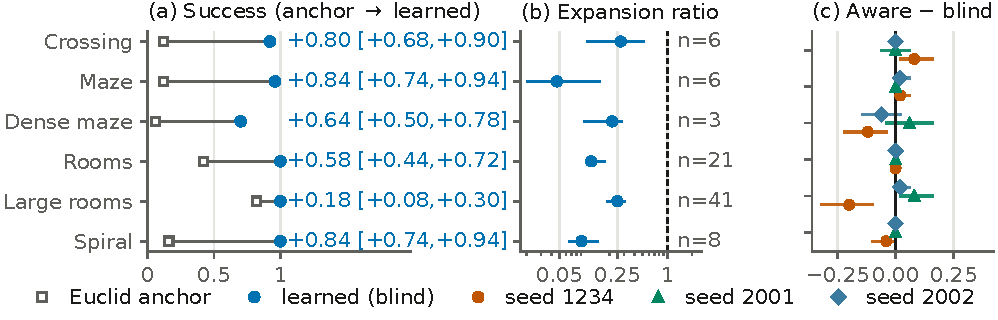
\includegraphics[width=0.98\textwidth]{figures/fig_dynamic_headline.pdf}
\caption{Dynamic zero-shot transfer of one fixed blind U-Net heuristic on the held-out 50-map-per-suite cohort. (a) Anchor and learned success per suite; labels give the paired mean delta (all six map-level 95\% CIs exclude zero; intervals in the appendix). (b) Matched-solved expansion ratios on a log axis, with map-level 95\% CIs; $n$ is the jointly solved count (dense maze, $n{=}3$, is descriptive). (c) Map-paired aware$-$blind success differences under the primary training seed. Per-seed tables and the cohort-disjointness check are in the appendix.}
\label{fig:dynamic}
\end{figure*}

\section{Problem Formulation and Learned-Heuristic Interfaces}

\textbf{Planning problems.} In the continuous setting, a point robot plans on a probabilistic roadmap \citep[PRM;][]{kavraki1996prm} built over a square world of side length 1.0 (2.0 for the large-room family); units are abstract. Each roadmap contains exactly 192 sampled nodes with $k{=}7$ nearest-neighbor connectivity; the start and goal are inserted as nodes 0 and 1, edges are validated by collision sampling, and worlds whose roadmap does not connect start to goal are rejected. Static search states are roadmap nodes; edge costs are Euclidean lengths; Euclidean distance to the goal is the anchor heuristic $h_0$. In the dynamic setting, obstacles move on deterministic trajectories, the search state is a pair $(v,t)$ of node and discrete time, and the planner may either traverse an edge (taking $\lceil \mathrm{len}/v_{\mathrm{agent}}\,dt \rceil$ steps) or wait one step; transitions are validated against the obstacle trajectories by sampled collision checks, cost is arrival time, and search runs to a horizon $t_{\max}$. In the discrete setting, agents plan on occupancy grids of $20{\times}20$ to $256{\times}256$ cells with Manhattan distance as the anchor.

\textbf{Supervision targets.} Static labels are exact graph-Dijkstra costs-to-go on the roadmap; dynamic labels are exact backward space--time Dijkstra values over $(v,t)$. Scalar models predict a nonnegative, capped residual $\hat\delta_\theta$ over the anchor from per-node feature tokens; field models predict a goal-conditioned residual raster (eight input channels: occupancy, free-space reachability, clearance, start and goal encodings, coordinates, and normalized anchor distance) sampled at node positions.

\textbf{Planner integrations.} Under \emph{additive} integration the planner orders states by $f(s) = g(s) + h_0(s) + \hat\delta_\theta(s)$, sacrificing admissibility for guidance; empirical path-cost ratios are reported wherever additive integration is used. Under \emph{focal (rank-only)} integration the anchor defines an admissible band $f \leq w \cdot f_{\min}$ \citep{pohl1970,pearl1982semiadmissible} and the learned prediction only orders expansions within the band; at $w{=}1.0$ node-optimality is untouched. In the restricted-observation study, learned predictions serve as exit values of a radius-bounded local subgraph and one Bellman backup over that subgraph, computed at inference, produces the heuristic; a scale factor is calibrated once on a disjoint block and then fixed.

\textbf{Transfer protocol.} Zero-shot transfer applies a trained-and-fixed heuristic to unseen maps and unseen map families with no target supervision. Few-shot adaptation draws $K$ labeled target maps and compares rank-8 LoRA \citep{hu2021lora}, full fine-tuning, and training from scratch from the same initialization and matched schedule. (In the compositional-mission study, $K$ instead denotes mission length; the two uses are flagged where they occur.)

\section{Experimental Setup}

\textbf{Environment families.} Continuous worlds are generated procedurally by our released generator (specification tables in the appendix). The static hard families are wall constructions: \emph{maze} and \emph{dense maze} (corridor mazes; the dense variant narrows the gap width to 0.115 of the side length), \emph{rooms} and \emph{large rooms} ($2{\times}2$ rooms formed by one vertical and one horizontal partition wall with one doorway each; the large variant doubles the side length), \emph{spiral} (four serpentine walls with alternating gap sides), and \emph{bugtrap} (a U-shaped pocket with a partially closed mouth). Static training uses the maze, rooms, and spiral families; dense maze, bugtrap, and large rooms are held out. Dynamic suites add 3--5 moving circular obstacles per world that sweep line segments with triangle-wave motion (radius 0.055--0.080, span 0.36--0.50, and period 0.14--0.30 of the horizon, per suite; exact per-suite parameters in the appendix), plus a \emph{crossing} open-arena suite as a timing control. The learned heuristic never observes a test map during training, and evaluation cohorts are generated from disjoint seed ranges; disjointness is checked by comparing world fingerprints (start, goal, and obstacle coordinates).

\textbf{Models.} Scalar models consume per-node token sequences (62 tokens: a summary token, 12 nearest-obstacle tokens, 48 ray tokens, and a goal token; 16 dimensions each) and include an MLP, an LSTM \citep{hochreiter1997lstm}, an ON-LSTM \citep{shen2019onlstm} (hidden 256, 2 layers; 1{,}252{,}481 parameters), and a Hierarchical Reasoning Model \citep[HRM;][]{wang2025hrm} (hidden 192, 2 layers, 4 heads; 2{,}158{,}529 parameters), including an adaptive-computation port \citep{graves2016act,banino2021pondernet}. Field models consume the eight-channel $64{\times}64$ raster and include a FiLM-conditioned U-Net \citep{ronneberger2015unet,perez2018film} (3{,}702{,}370 parameters), a field HRM (4{,}016{,}642), and a field ON-LSTM (1{,}448{,}578); dynamic variants append $W$ future-occupancy channels ($W{=}8$ aware, $W{=}0$ blind). All models train with AdamW (learning rate $2{\times}10^{-4}$, weight decay $10^{-4}$, batch 256, gradient clipping 1.0) on a smooth-L1 residual loss with cap 4.0; complete architecture and optimizer tables are in the appendix. Within each direct architecture comparison, models are trained under one matched recipe on identical data.

\textbf{Evaluation.} Each suite is evaluated at a per-suite expansion budget selected by calibration: candidate budgets are swept on the evaluation worlds, and the lowest budget at which the anchor baseline's success falls in a discriminative band (roughly 0.25--0.62 observed across formal static cells) is fixed as the binding budget before learned methods are compared. Success means reaching the goal within the budget; the appendix reports success as a function of budget up to $4\times$ the binding budget, derived exactly from recorded expansion counts. Search effort is the \emph{matched-solved expansion ratio}: the median over jointly solved maps of the per-map ratio of learned to anchor expansions. Because it conditions on joint success, it can favor a method that solves only easier maps; success is therefore always reported first, and empirical path-cost ratios are reported separately wherever additive integration is used.

\textbf{Statistics.} Success comparisons use paired tests (McNemar within suites) with Benjamini--Hochberg correction applied within each experiment's family of suite-level comparisons; adjusted values are reported as $q$. Interval estimates are percentile bootstraps with 10{,}000 resamples; the resampling unit is the evaluation map, and repeated adaptation or model seeds are averaged within maps before resampling. Success deltas in Figure~\ref{fig:dynamic} are paired map-level bootstrap intervals. Unless noted, continuous experiments use one primary training seed; the dynamic primary result additionally reports two retrained seeds, and the mission and refiner experiments use three-seed grids.

\section{Dynamic Zero-Shot Transfer}

\textbf{Setting and fixed-model protocol.} The dynamic experiment uses the six moving-obstacle suites with exact space--time labels; the heavy training run collects 53 usable training worlds (a world is usable if it builds, its roadmap connects start to goal, and the space--time problem is solvable from the start at $t{=}0$) totaling 1{,}129{,}536 supervised state samples. To remove selection over architectures, the primary analysis fixes \emph{one} learned heuristic for every suite: the field U-Net \emph{blind} twin, which receives no future-motion input. This model was fixed---architecture, weights, integration, and per-suite budgets---after the original 20-map evaluation but \emph{before the 50-map confirmation cohort was generated}; the confirmation cohort's generation seed was chosen in advance and is map-disjoint from every earlier cohort by the fingerprint check. The blind heuristic receives only current-time occupancy channels; the space--time planner and collision checker always use the true deterministic trajectories when validating $(v,t)$ transitions, so the ablation changes only the heuristic's input.

\textbf{Confirmation result.} On the held-out 50-map-per-suite cohort, the fixed blind U-Net raises success on all six suites: deltas $+0.18$ to $+0.84$, with every paired map-level 95\% CI excluding zero, and matched expansion-ratio medians of 0.047--0.273---a 73--95\% reduction in search effort on jointly solved maps (Figure~\ref{fig:dynamic}; jointly solved counts 3--41 per suite). The original 20-map cohort gives the same picture (deltas $+0.20$ to $+0.75$; medians 0.087--0.246; appendix), so the success result holds on two disjoint evaluation cohorts.

\textbf{Training-seed robustness.} Two additional full training pipelines with independent seeds, evaluated on the same held-out cohort, reproduce the success result: across the three seeds, 17 of 18 seed--suite paired CIs exclude zero (deltas $+0.10$ to $+0.88$; the single crossing interval is a near-ceiling large-rooms cell where the anchor already solves 0.82). Effort magnitudes are seed-stable on three suites (medians 0.047--0.135 under every seed) and seed-variable on the other three (0.216--0.625 across seeds); we therefore quote effort as across-seed ranges on those suites. We distinguish this training-seed robustness from the evaluation-cohort replication above: the retrained models are evaluated on the same 50 maps.

\textbf{Future-window inputs provide no consistent benefit.} The primary model above is already the blind twin, so the gains require no future-motion input; the twin study quantifies the contrast directly. Aware and blind twins differ in exactly one input: eight channels of ground-truth future occupancy. On the held-out cohort the contrast is suite-dependent in both directions and unstable across training seeds: of the 18 suite-level contrasts from the three seeds, two significantly favor the aware twin, two the blind twin, and fourteen neither. The significant cells fall in different suites for different seeds---large rooms flips from significantly blind-better ($-0.200$ $[-0.320,-0.100]$) under one seed to significantly aware-better ($+0.080$ $[+0.020,+0.160]$) under another (Figure~\ref{fig:dynamic}(c) shows the primary seed; per-seed tables in the appendix). The original run's 24 suite-by-backbone cells point the same way (one uncorrected significant cell favors aware, seven favor blind), and after full fine-tuning on $K{=}16$ target maps, eight of nine map-level success differences are non-positive with the sole positive interval including zero. We report a failure to observe a systematic future-window benefit under deterministic dynamics---not equivalence, and not harm; stochastic motion is untested.

\section{Why Transferred Heuristics Help or Fail}

\textbf{Static family transfer.} The same transfer pattern holds without dynamics. On the six calibrated static suites---trained on maze, rooms, and spiral; evaluated additionally on the held-out dense maze, bugtrap, and large rooms---the transferred field HRM solves 0.75--1.00 of test maps against anchor success of 0.25--0.58, with BH-adjusted $q$ values ranging from below 0.001 to 0.025 on four suites and matched expansion ratios of 0.521--0.850. Pooled models trained on the three source families also improve success on every held-out family before any target labels are used.

\textbf{Supervised target.} On the calibrated hard static maps, a pooled ON-LSTM scalar residual model raises hard-maze success from 0.525 to 1.000 over the anchor ($q=4.3\times10^{-11}$), while the parameter-matched scalar HRM collapses to a constant prediction at the residual cap and merely matches the baseline; lower learning rates and a soft-cap variant reproduce the collapse. Keeping the HRM and changing only the supervised target to the raster residual field raises hard-maze success from 0.625 to 0.975 ($q=3.4\times10^{-4}$); a subsequent stage shows a well-trained scalar HRM is also viable (per-suite ratios 0.427--0.822). These controls localize the failure to the target and optimization path: value fields are not intrinsically necessary, and the HRM is not intrinsically unsuitable, but the target choice changed the outcome while the model family was held fixed.

\begin{figure}[t]
\centering

\includegraphics[width=0.98\columnwidth]{figures/fig2_integration.pdf}
\caption{Planner-integration results in discrete and continuous settings. Discrete grids (tight Manhattan anchor): additive learned magnitude is at or below baseline, while the same trained predictions reduce expansions by 6--15\% as a within-band ranker. Continuous roadmaps (loose Euclidean anchor): additive guidance reduces matched expansions by 15--48\%, and rank-only variants recover less.}
\label{fig:integration}
\end{figure}

\textbf{Planner integration.} The two substrates give opposite answers about the useful interface (Figure~\ref{fig:integration}). On continuous roadmaps, additive residuals exploit the gap the Euclidean anchor leaves: field-HRM ratios are 0.521--0.850 at empirical path-cost ratios of roughly 1.02--1.14, while rank-only variants stay closer to plain anchor search. On discrete grids the learned signal is demonstrably informative---the pooled residual correlates 0.987--0.994 with the true residual across map sizes---but its magnitude is scale-flat (predicted-to-true mean falls from 0.73 to 0.19 as maps grow), and every additive configuration in the controlled 22-suite run is at or below its matched baseline. Reusing the \emph{same} trained predictions only to rank expansions inside a $w{=}1.0$ focal band cuts expansions by 6--15\% in the tested cells with no observed success regression \citep{chrestien2023rank}. In this discrete control, changing only the integration recovered the useful ordering signal; we interpret the cross-substrate pattern---additive helps against a loose anchor, ranking against a tight one---as a hypothesis supported by these results rather than an isolated cause.

\textbf{Oracle integration control.} A final control removes learning entirely. An exact value ranker paired with a fresh certifier search that discards the incumbent's work loses all six primary comparisons (141.2 versus 129.7 mean expansions); sharing a single search queue and $g$-state---which changes no oracle values---wins all six (122.8). Oracle-quality values alone therefore do not determine the outcome; the search-state interface does. A negative transfer or architecture result is uninterpretable until the target and integration are validated.

\section{Few-Shot Adaptation}

\begin{figure}[t]
\centering
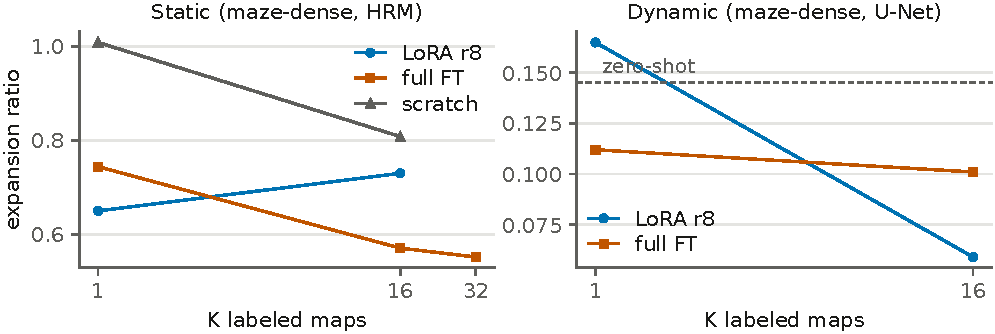
\includegraphics[width=0.98\columnwidth]{figures/fig3_transfer.pdf}
\caption{Representative static (left) and dynamic (right) adaptation curves for the maze-dense targets. On the static target, rank-8 LoRA preserves the transferred gain at $K{=}1$ while full fine-tuning can fail early and often wins by $K{=}8$--16; on the dynamic target, where a single map supplies tens of thousands of labeled states, the low-label failure mode is not observed. Quoted inference in the text is map-clustered; the full per-cell grid is in the appendix.}
\label{fig:transfer}
\end{figure}

\textbf{Scarce static labels.} At $K{=}1$ on the dense-maze target, rank-8 LoRA retains the zero-shot gain: map-level ratio 0.686 (95\% CI $[0.590,0.774]$) with success delta $+0.467$ ($[+0.300,+0.633]$). Unconstrained updates are unstable in the same regime: full fine-tuning on large rooms at $K{=}1$ reaches ratio 1.293 ($[1.170,1.503]$), and training from scratch on dense maze is significantly harmful (success $-0.167$ $[-0.300,-0.047]$; ratio 1.035). At low supervision the transferred model is an asset that the update rule can preserve or destroy (Figure~\ref{fig:transfer}, left).

\textbf{Full fine-tuning improves at larger $K$.} By $K{=}8$--16 full fine-tuning often overtakes LoRA; on dense maze at $K{=}16$ the map-level intervals are disjoint (0.610 $[0.549,0.670]$ versus 0.786 $[0.694,0.891]$). A matched-compute ablation compares bounded and unbounded LoRA across 27 cells: the map-level ratio differences have median 0.0000 (standard deviation 0.0077; maximum 0.037), so the near-identical curves suggest the output clamp is not the primary cause of the LoRA plateau. LoRA is not universally protective either: on bugtrap it degrades significantly by $K{=}32$ (ratio 1.153 $[1.012,1.523]$).

\textbf{Dynamic maps supply many labels per map.} The heavy dynamic run collects 1{,}129{,}536 supervised $(v,t)$ samples from 53 training worlds---on the order of $2\times10^{4}$ labeled states per world (exact collection arithmetic in the appendix). At dynamic $K{=}1$, full fine-tuning is not systematically catastrophic and LoRA continues to improve rather than merely preserve the base (Figure~\ref{fig:transfer}, right). Scratch models can post attractive solved-only ratios while solving fewer maps, so success leads those comparisons. This behavior is consistent with the effective number of supervised states differing by two orders of magnitude between the static and dynamic $K{=}1$ conditions; the two settings also differ in other respects, so we state this as an association rather than an isolated cause.

\section{Scope and Boundary Results}

\textbf{Discrete transfer.} In the complete pooled-multitask grid run, the pooled HRM base improves mean success from 0.591 to 0.612 with lower mean expansions (descriptive); task-specific adapters do not improve broadly. A 3--8-seed pilot on selected 128- and 192-cell maps finds 6--15\% expansion reductions at $w{=}1.0$ with equal or higher observed success; a full-suite confirmation has not been run.

\textbf{Adapter composition did not improve the pooled model.} Interpolating 16 single-family rank-8 adapters by target descriptor routes to the correct family axis (own-axis mass 0.986--0.998), yet map-paired composition never significantly beats the pooled zero-shot model and is significantly worse in two of six cells (ratio deltas up to $+0.098$ $[+0.076,+0.123]$); weight-space and prediction-space mixtures are nearly identical \citep{wortsman2022soups,ilharco2022task}.

\textbf{Architecture and hierarchical depth.} Architecture rankings differ across the tested tasks and input representations: the U-Net is often strongest in the dynamic field study, the HRM holds the lowest single-suite dynamic ratio, and the ON-LSTM leads the early calibrated scalar stage. In compositional multi-leg missions constructed with verified oracle headroom (mission length $K \in \{2,4,8\}$; six learned configurations, three seeds, 54{,}450 evaluation rows), no structured model beats the MLP at two depths with a non-decreasing gap, forced extra recurrent compute yields flat curves, and learned halting moves \emph{opposite} to the depth hypothesis (mean would-halt steps 6.79/7.01/5.30 at $K{=}2/4/8$; map-level $\rho=-0.578$, stratified permutation $p=5\times10^{-5}$). Global-input models do separate from the MLP at shallow missions (ratios ${\approx}$0.67--0.87 in two of three configurations). Five of 33 recurrent cells collapse to constant predictions and are treated as optimization failures rather than capacity estimates. Follow-up experiments on persistent memory, iterative refinement \citep{tamar2016vin,lee2018gppn}, hierarchical substitution, and persistent planning-time state are also negative (persistent carry worsens frontier ranking; MRR delta $-0.0294$ $[-0.0598,-0.0030]$); full gate tables and figures are in the appendix. These are formulation-specific negatives, not claims that recurrence, memory, or hierarchy are universally ineffective \citep{jolicoeur2025trm,czechowski2021subgoal}.

\textbf{Restricted-observation transfer.} A final static study restricts the learned model to a radius-0.20 local subgraph of the roadmap, trained from behavior-derived returns rather than shortest-path labels, and integrates it through one inference-time Bellman backup over that subgraph. Under a preregistered comparison on a disjoint 144-map cohort, this local MLP reduces pooled expansions against the complete-map field HRM by 12.96 (95\% CI $[-16.30,-9.74]$; 109/3/32 wins/ties/losses; every suite mean lower) at better empirical path quality (mean/max cost ratios 1.024/1.162 versus 1.031/1.335), and a separate $w{=}1.10$ bounded control passes all 144 per-instance suboptimality certificates. Sequential ablations attribute the sign change to the backup itself: the same trained model loses by $+16$ expansions under static insertion and wins after one backup. The study is static, uses one model seed and cohort, carries no formal bound on the direct arm, and its prototype feature construction is slower in wall time; full ladder, calibration, and timing tables are in the appendix.

\section{Related Work}

\textbf{Learned guidance for search.} Learned heuristics have been trained by bootstrapping \citep{arfaee2011bootstrap}, oracle imitation \citep{bhardwaj2017sail}, differentiable search \citep{yonetani2021neuralastar}, transformer-based grid guidance \citep{kirilenko2023transpath}, supervised classical-planning objectives \citep{ferber2020neural}, and ranking objectives \citep{chrestien2023rank}. These works evaluate primarily on maps drawn from the training distribution and each commit to one planner interface; the main difference in our work is that we hold the classical planner fixed, evaluate cross-family and dynamic transfer of the same trained models, and compare additive against rank-only integration of identical predictions \citep{pohl1970,pearl1982semiadmissible,aine2016mha}.

\textbf{Dynamic, real-time, and motion planning.} The dynamic substrate follows space--time and safe-interval search \citep{silver2005cooperative,phillips2011sipp}. The restricted-observation study is related to real-time heuristic search \citep{korf1990rta} and local value updates in Real-Time Adaptive A\textsuperscript{*} \citep{koenig2006rtaa}; its one-step backup also resembles a single value-iteration-network update \citep{tamar2016vin,lee2018gppn} and neural algorithm execution more broadly \citep{velickovic2021nar}. Unlike those methods, the backup here is applied once, at inference, over a radius-bounded subgraph, purely to integrate a transferred prediction. Learned samplers and end-to-end motion planners \citep{ichter2018sampling,qureshi2019mpnet} replace or augment the planner itself; we retain a fixed classical planner and learn only its guidance, which is what makes heuristic transfer measurable on a PRM \citep{kavraki1996prm}.

\textbf{Adaptation and recursive architectures.} LoRA \citep{hu2021lora}, model soups \citep{wortsman2022soups}, and task arithmetic \citep{ilharco2022task} motivate the low-rank and composition studies; the contribution here is not the use of LoRA but the comparison of low-rank against full-rank updates as a function of planning-label availability. HRM \citep{wang2025hrm}, adaptive computation \citep{graves2016act,banino2021pondernet}, and simplified recursive models \citep{jolicoeur2025trm} motivate the architecture experiments; our results concern heuristic regression and planner integration rather than the benchmark claims of those architectures.

\section{Limitations}

Most continuous primary results are local single-GPU validations with one primary training seed, and several experiments reuse trained bases or test maps rather than constituting independent replications. The dynamic primary result holds on two disjoint evaluation cohorts and is robust to two additional training seeds under a pre-specified protocol, but the smallest jointly solved cell remains three maps (dense maze), matched-effort magnitudes vary by seed on three of six suites, and a per-suite best-configuration view reported in the appendix is post-hoc. The discrete rank-only result covers selected cells with 3--8 seeds, not the full 22-suite grid. Map-clustered reanalysis supports the quoted adaptation and architecture conclusions, but not every exploratory table has been regenerated at that grain, and no equivalence tests were run.

The restricted-observation confirmation is static, uses one model seed and one 144-map cohort, and tests whether the transferred signal survives input restriction; it is not evidence about moving obstacles. Its model is locally restricted but the planner still knows the roadmap; this is not map-free sensing. The direct operating point has no formal suboptimality bound, while the certified control is slower, and the prototype feature construction is slower in wall time than complete-map inference despite fewer expansions.

Dynamic obstacles are deterministic, and the work does not cover stochastic prediction, kinodynamic constraints, multi-agent coupling, physical robots, or environments beyond 2-D single-agent navigation. All environments are synthetic; establishing comparability with standardized external benchmarks remains open. Negative results are failures to observe improvement under the pre-specified protocols, not universal rejections of future information, composition, recurrence, memory, or hierarchy. Safety-critical deployment would additionally require uncertainty-aware motion models, collision guarantees, and end-to-end validation.

\section{Conclusion}

Across discrete grids and continuous roadmaps, learned heuristics transferred to unseen maps, unseen map families, and unseen dynamic environments---and whether that transfer improved search depended on the supervised target, the planner interface, and the amount of target supervision, more consistently than on the model family. A single trained U-Net heuristic, fixed in advance and given no future-motion input, improved success on every held-out dynamic suite while cutting matched search effort by 73--95\%. In the static low-label regime, low-rank adaptation protected the transferred model where full fine-tuning destroyed it, and the ordering reversed as labels grew. The practical implication is that learned planning heuristics should be evaluated---and deployed---jointly with their planner interface and supervision regime, not as models in isolation.

\bibliography{references}

% AAAI-27 requires the reproducibility checklist to be uploaded separately
% in the designated submission field; it should not be included in this PDF.

\end{document}
